\section{The effects of smoothing}
\label{sec:smooth}

Here we present comparisons between smoothing methods used in image creation first comparing Gaussian and spline kernel smoothing and then the differences between smoothing and ignoring smoothing.

\subsection{Comparing kernel averaging to Gaussian smoothing}

\begin{figure*}
	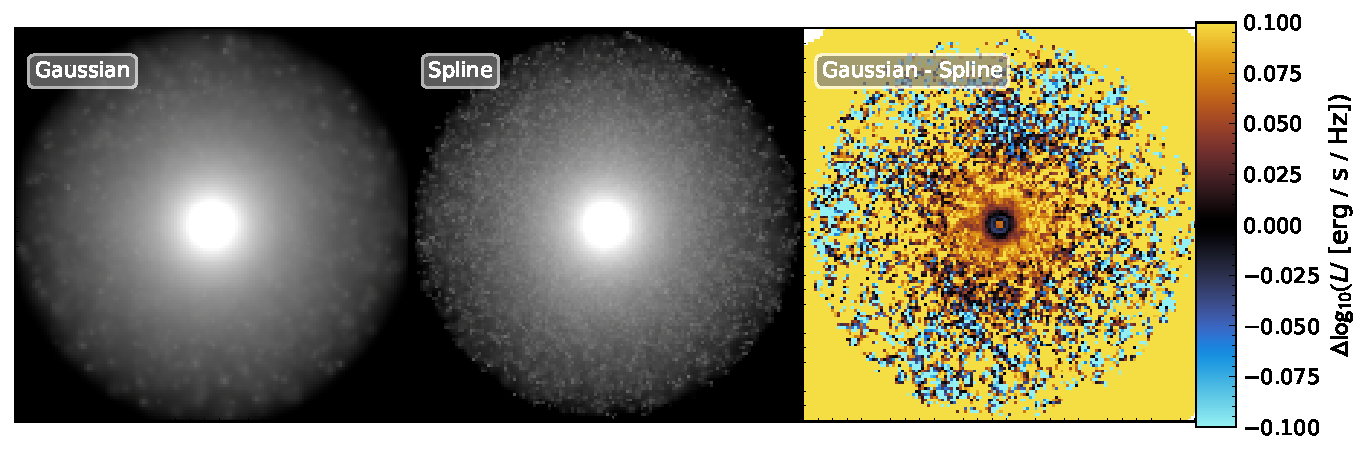
\includegraphics[width=\linewidth]{Figures/ComparisonImageCreation_Residual_FAKE.TH.FUV_5.0_sim_Total_default.pdf}
    \caption{A comparison of logscaled stacked images produced using the Gaussian smoothing method (left), spline kernel method (middle) and a residual image showing the difference between the log of the two methods images. The images themselves are stacks in the far UV of all galaxies in the \flares\ sample (irrespective of completeness).}
    \label{fig:imgtyperesi}
\end{figure*}

\fig{imgtyperesi} shows a comparison between the Gaussian and spline smoothing methods. Qualitatively it can be seen the Gaussian method results in a smoother light distribution due to the indefinite boundaries of the Gaussian smoothing kernel, this spreads light beyond the `extent' given by the SPH kernel. The spline method produces a more granular image with clearer small structures at the outskirts of the FOV. The residual image shows that the Gaussian method's spreading of light leads to differences at large radii where the Gaussian image is brighter due to the spreading of light. However, this does not mean the Gaussian image is consistently more luminous at large radii, compact structures at large radii in the spline image have more concentrated emission causing these regions to out shine the Gaussian image. This effects is also noticeable in the centre of the image where there is a ring of spline dominated pixels due to this concentration of light. These effects are however minimal with each image differing at most by 0.1 dex. 

\begin{figure}
	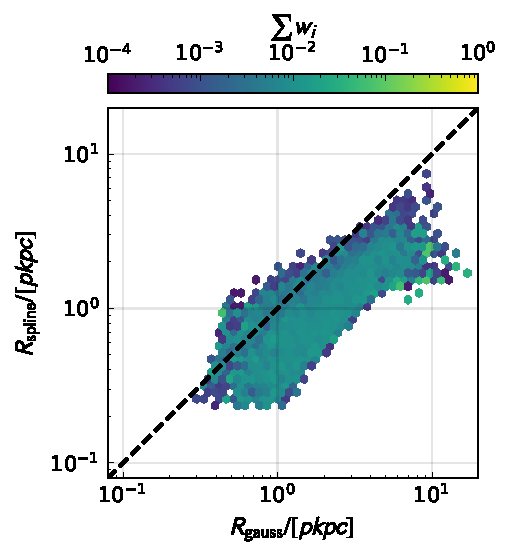
\includegraphics[width=\columnwidth]{Figures/ComparisonImageCreation_HLR_FAKE.TH.FUV_5.0_sim_Total_default.pdf}
    \caption{A comparison between the sizes of galaxies measured using the pixel method from the spline (y-axis) and Gaussian (x-axis) smoothing methods. The dashed line represents a 1:1 relation. In this plot we do not differentiate between the compact and diffuse galaxy populations and only present the full complete sample.}
    \label{fig:imgtypehlr}
\end{figure}

We further show the effects of smoothing method in \fig{imgtypehlr} where we compare the measured sizes of galaxies in each method. In the vast majority of cases the Gaussian smoothing results in a larger perceived size due to the increased spread of a single stellar particle's luminosity. The instances where the spline method yields larger sizes are dominated by smaller galaxies where the dilution of the Gaussian method causes structures to occupy more pixels relative to the more concentrated spline method and thus a larger area is used in the pixel driven size calculation. It should be noted here that the spline method produces a better agreement with observations with the Gaussian method producing size-luminosity relations which overestimate galaxy sizes relative to observations.

\subsection{Smoothing vs no smoothing}


\begin{figure}
	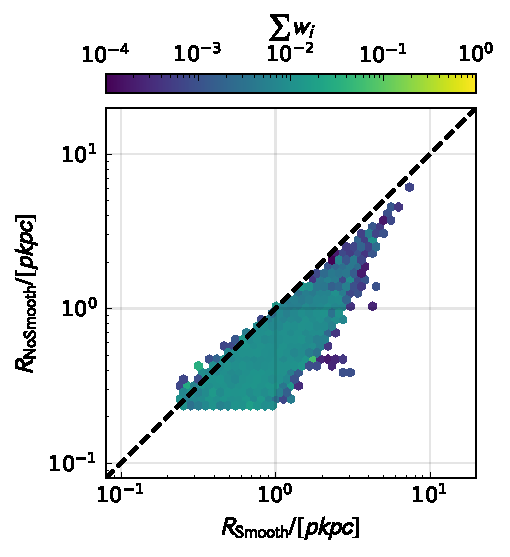
\includegraphics[width=\columnwidth]{Figures/ComparisonHalfLightRadiusSmoothing_FAKE.TH.FUV_5.0_sim_Total_default.pdf}
    \caption{A comparison between sizes of galaxies measured using the pixel method from dust attenuated images with and without smoothing of the stellar particles. The dashed line represents a 1:1 relation. In this plot we do not differentiate between the compact and diffuse galaxy populations and only present the full complete sample.}
    \label{fig:nosmooth}
\end{figure}

In \fig{nosmooth} we compare the spline smoothing method to galaxy sizes measured from images where no smoothing has been performed on the stellar particles. In some cases there is minimal difference between the smoothed and unsmoothed measurements, particularly for compact galaxies where the stellar kernels themselves are very small resulting in minimal smoothing. In the vast majority of cases the smoothing increases the measured size, with the most diffuse incomplete galaxies (transparent distribution) extending to much larger sizes when smoothed.

% Commented out for now... 

% \section{Sample variations}
% \label{sec:sample-vary}

% Here we present the main results of the paper, the attenuated size-luminosity relation and redshift evolution of size ignoring the completeness limits placed on the \flares\ sample to ensure a complete robust sample (galaxies are still required to have $N_\star>100$). Many of the galaxies that were omitted by these limits from the analysis in the main body of the paper pose a distinct challenge to observations as many fall below the deepest surface density limits of modern surveys. In addition to the observational limitations this is also a regime where structure identification methods used in simulations begin to struggle producing less robust structures, therefore these results should be interpreted with care and are included here only for completeness. 

% \subsection{Size-Luminosity}
% \label{sec:sample:incom_size}

% \begin{figure*}
% 	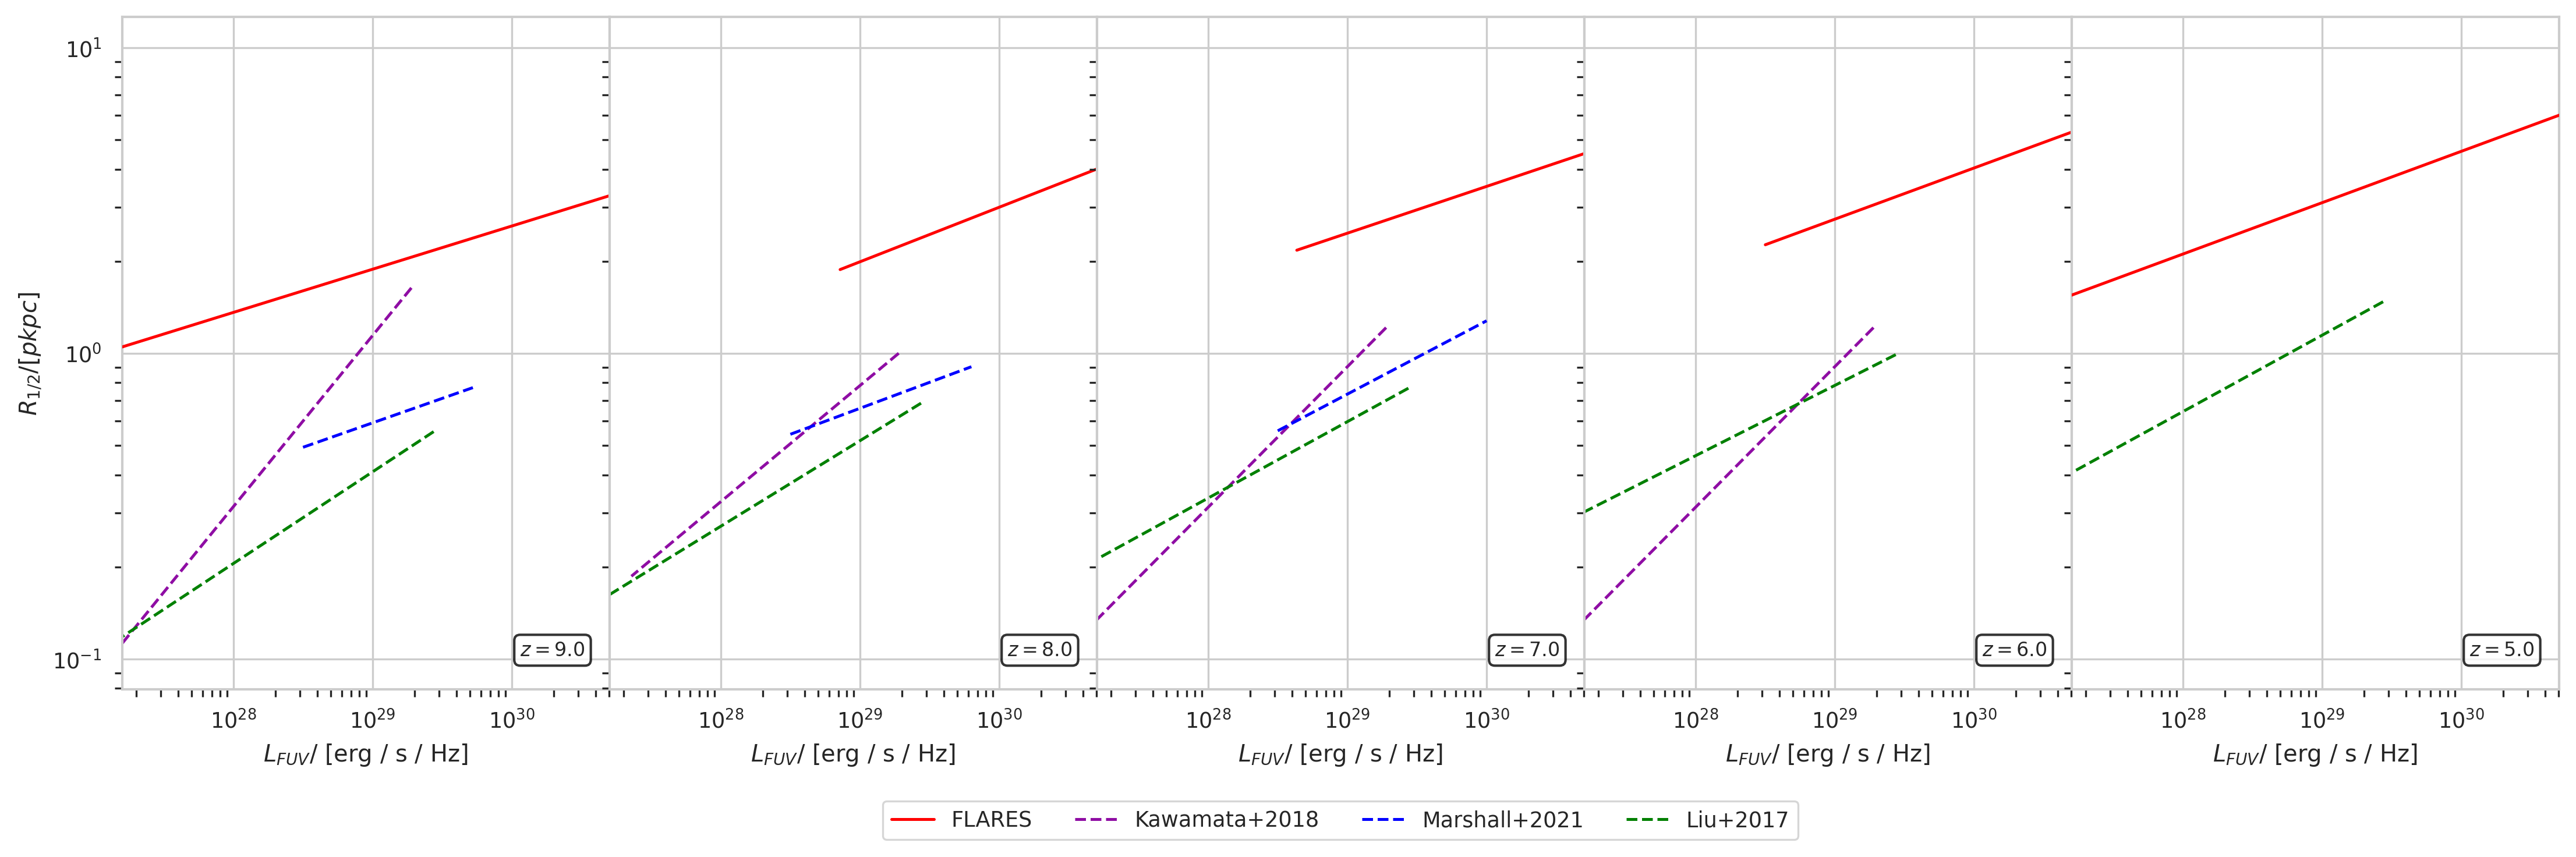
\includegraphics[width=\linewidth]{Figures/FitHalfLightRadius_pix_FAKE.TH.FUV_sim_Total_default_All.pdf}
%     \caption{A reproduction of \fig{fits_obscomp} ignoring completeness limits (galaxies are still required to have $N_\star>100$).}
%     \label{fig:all_size_lumin}
% \end{figure*}

% The fits to the attenuated size-luminosity relation vary significantly more with evolving redshift in the absence of sample cuts. This is shown in \fig{all_size_lumin} where \fig{fits_obscomp} has been reproduced, with the inclusion of the comparison fits for context. At the highest redshifts this leads to a negatively sloped size-luminosity relation which flattens with increasing redshift. This is due to the extremely numerous low luminosity diffuse galaxies that populate the upper left portion of the size-luminosity relation. As these galaxies evolve many more of them enter the compact population and increase significantly in size causing the evolution from negative to positive slope evident from left to right. 

% \subsection{Redshift Evolution}
% \label{sec:incom_evo}

% \begin{figure}
% 	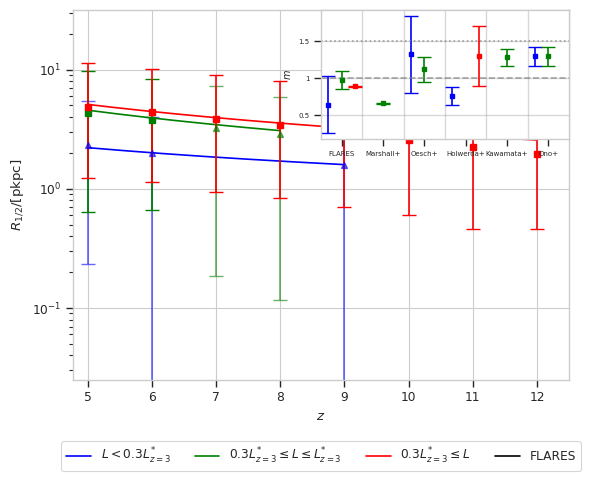
\includegraphics[width=\columnwidth]{Figures/Violin_ObsCompHalfLightRadius_evolution_pix_FAKE.TH.FUV_sim_default_NonComplete.pdf}
%     \caption{A reproduction of \fig{evo} ignoring completeness limits (galaxies are still required to have $N_\star>100$).}
%     \label{fig:all_evo}
% \end{figure}

% In the redshift evolution we see negligible change in the sample capped at $L^{*}_{z=3}$ and high luminosity samples as these galaxies are minimally effected by the completeness limits. The low luminosity sample however now contains significantly more galaxies, especially at early times. The effects of this can be seen in \fig{all_evo} where the low luminosity sample exhibits a far flatter evolution which in fact now falls in agreement with \cite{Holwerda_2015}. This can be explained by the fact galaxies in this luminosity regime are intrinsically diffuse at their birth and thus evolve much slower if they remain in the diffuse and dim population of galaxies.

\section{Size-luminosity relation wavelength variation}

In this appendix we present the fitting parameters for the wavelength evolution of the size-luminosity relation shown in \fig{colors}.

\label{sec:bandtable}

\begin{table*}
\begin{center}
\begin{tabular}{ c | c | c | c | c | c | c | c | c | c }
 \hline
 Redshift ($z$) & \multicolumn{2}{|c|}{9} & \multicolumn{2}{|c|}{8} & \multicolumn{2}{|c|}{7} \\ \hline
 Band & $R_0$ & $\beta$& $R_0$ & $\beta$ & $R_0$ & $\beta$ \\ \hline
 FUV 
 & 0.793 +/- 0.019 & 0.519 +/- 0.026
 & 0.842 +/- 0.012 & 0.319 +/- 0.013
 & 1.126 +/- 0.011 & 0.290 +/- 0.008 \\
 MUV 
 & 0.773 +/- 0.020 & 0.493 +/- 0.026
 & 0.821 +/- 0.012 & 0.313 +/- 0.013
 & 1.070 +/- 0.011 & 0.263 +/- 0.008 \\
 NUV 
 & 0.777 +/- 0.021 & 0.485 +/- 0.026
 & 0.813 +/- 0.013 & 0.296 +/- 0.014 
 & 1.020 +/- 0.013 & 0.211 +/- 0.009 \\
 U 
 & 0.687 +/- 0.017 & 0.434 +/- 0.026 
 & 0.743 +/- 0.011 & 0.262 +/- 0.014 
 & 0.878 +/- 0.011 & 0.092 +/- 0.010 \\
 B 
 & 0.660 +/- 0.014 & 0.428 +/- 0.025 
 & 0.704 +/- 0.010 & 0.133 +/- 0.014 
 & 0.854 +/- 0.010 & -0.017 +/- 0.010 \\
 V 
 & 0.702 +/- 0.018 & 0.375 +/- 0.024 
 & 0.689 +/- 0.013 & 0.022 +/- 0.014 
 & 0.823 +/- 0.011 & -0.114 +/- 0.009 \\
 R
 & 0.573 +/- 0.011 & 0.397 +/- 0.027 
 & 0.638 +/- 0.008 & 0.154 +/- 0.014
 & 0.765 +/- 0.009 & -0.030 +/- 0.011 \\
 I
 & 0.598 +/- 0.019 & 0.178 +/- 0.026 
 & 0.601 +/- 0.013 & -0.110 +/- 0.015 
 & 0.763 +/- 0.011 & -0.167 +/- 0.009 \\
 Z
 & 0.558 +/- 0.015 & 0.229 +/- 0.027 
 & 0.583 +/- 0.011 & -0.077 +/- 0.015 
 & 0.715 +/- 0.010 & -0.186 +/- 0.010 \\
 Y
 & 0.595 +/- 0.014 & 0.312 +/- 0.026 
 & 0.616 +/- 0.010 & -0.000 +/- 0.014 
 & 0.715 +/- 0.010 & -0.183 +/- 0.010 \\
 J
 & 0.532 +/- 0.017 & 0.090 +/- 0.027 
 & 0.525 +/- 0.011 & -0.220 +/- 0.015 
 & 0.698 +/- 0.010 & -0.228 +/- 0.009 \\
 H
 & 0.476 +/- 0.017 & -0.035 +/- 0.027 
 & 0.503 +/- 0.011 & -0.268 +/- 0.014
 & 0.688 +/- 0.010 & -0.250 +/- 0.008 \\
 \hline
\end{tabular}
\caption{The fitting results for \eq{size_lumin_fit} for $z=7-9$ and all rest frame bands in \fig{colors}. $R_0$ is a normalisation factor, $\beta$ is the slope of the size-luminosity relation and $N$ is the number of galaxies used in each fit.}
\label{tab:colorrfit1}
\end{center}
\end{table*}

\begin{table*}
\begin{center}
\begin{tabular}{ c | c | c | c | c | c | c}
 \hline
 Redshift ($z$) & \multicolumn{2}{|c|}{6} & \multicolumn{2}{|c|}{5} \\ \hline
 Band & $R_0$ & $\beta$ & $R_0$ & $\beta$ \\ \hline
 FUV 
 & 1.370 +/- 0.007 & 0.279 +/- 0.004 
 & 1.692 +/- 0.006 & 0.300 +/- 0.003 \\
 MUV 
 & 1.326 +/- 0.007 & 0.256 +/- 0.004
 & 1.639 +/- 0.006 & 0.280 +/- 0.003 \\
 NUV 
 & 1.315 +/- 0.008 & 0.238 +/- 0.004
 & 1.627 +/- 0.006 & 0.261 +/- 0.003 \\
 U 
 & 1.218 +/- 0.007 & 0.184 +/- 0.004
 & 1.514 +/- 0.006 & 0.215 +/- 0.003 \\
 B 
 & 1.227 +/- 0.007 & 0.111 +/- 0.004 
 & 1.526 +/- 0.005 & 0.149 +/- 0.003 \\
 V 
 & 1.285 +/- 0.008 & 0.060 +/- 0.004 
 & 1.604 +/- 0.006 & 0.104 +/- 0.002 \\
 R
 & 1.106 +/- 0.005 & 0.124 +/- 0.005 
 & 1.383 +/- 0.004 & 0.156 +/- 0.003 \\
 I
 & 1.238 +/- 0.008 & 0.021 +/- 0.004 
 & 1.554 +/- 0.006 & 0.069 +/- 0.002 \\
 Z
 & 1.155 +/- 0.007 & 0.013 +/- 0.004 
 & 1.455 +/- 0.005 & 0.064 +/- 0.002 \\
 Y
 & 1.143 +/- 0.007 & 0.019 +/- 0.004 
 & 1.439 +/- 0.005 & 0.061 +/- 0.002 \\
 J
 & 1.161 +/- 0.007 & -0.023 +/- 0.004 
 & 1.455 +/- 0.005 & 0.024 +/- 0.002 \\
 H
 & 1.146 +/- 0.007 & -0.053 +/- 0.004
 & 1.430 +/- 0.005 & -0.004 +/- 0.002 \\
 \hline
\end{tabular}
\caption{The fitting results for \eq{size_lumin_fit} for $z=6-5$ and all rest frame bands in \fig{colors}. $R_0$ is a normalisation factor, $\beta$ is the slope of the size-luminosity relation and $N$ is the number of galaxies used in each fit.}
\label{tab:colorrfit2}
\end{center}
\end{table*}